\documentclass[
	classe=$2^{de}$,
	headerTitle=Activité
]{exercice}

\begin{luacode}
	position = { x = 0, y = 1 }
	vitesse =  { x = 0, y = 0 }
	acceleration = { x = 1, y = 0.5 }

	function update_position()
	position.x = position.x + vitesse.x
	position.y = position.y + vitesse.y
	end

	function update_vitesse()
	vitesse.x = vitesse.x + acceleration.x
	vitesse.y = vitesse.y + acceleration.y
	end

	function draw_position(k, args)
	args = args or ""
	tex.print("\\node[", args, "] at (", position.x, ",", position.y, ") {×};")
	tex.print("\\node[above,", args, "] at (", position.x, ",", position.y, ") {$V_{", k, "}$};")
	end

	function draw_vitesse(k, args)
	args = args or ""
	tex.print("\\draw[->,", args, "] (", position.x, ",", position.y, ") -- node[above] {$\\vec{v_{", k, "}}$} ++(",vitesse.x ,",",vitesse.y ,");")
	end
\end{luacode}

\title{Activité : Position d'un avion}

% \newcommand{\makeCorrection}{}
\begin{document}

\maketitle

On veut simuler la position d'un avion en vol. On simplifiera ici nos calculs : on se place en 2 dimensions, et on suppose que la position de l'avion évolue de seconde en seconde (plutôt que continuellement).

\section{Sans gravité}

On veut déterminer deux variables liées à l'avion : sa \textit{position}, et sa \textit{vitesse}.

\begin{itemize}
	\item Le point $V$ est la position initiale de l'avion.
	\item La vitesse est représentée sur le graphique par le vecteur $\vec{v}$.
	\item À chaque seconde, l'avion est déplacé de $\vec{v}$.
\end{itemize}

Sur le quadrillage ci-dessous, placer les quatres prochaine positions de l'avion, en indiquant à chaque fois sa vitesse.

\begin{center}
	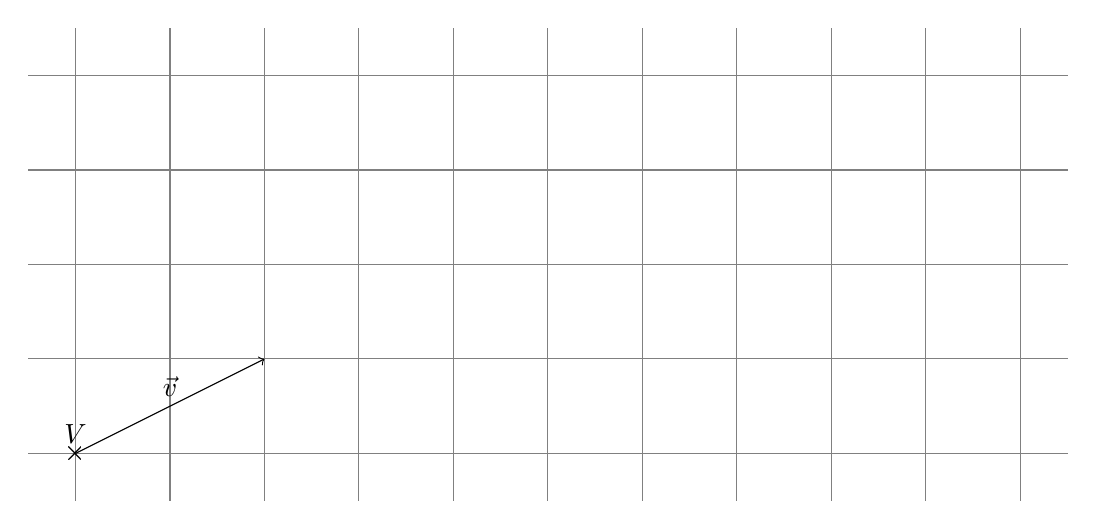
\begin{tikzpicture}[scale=1.2]
		\coordinate (AvionPosition) at (0,0);

		\draw[thin,gray] (-0.5,-0.5) grid (10.5,4.5);

		\node at (AvionPosition) {×};
		\node[above] at (AvionPosition) {$V$};
		\draw[->] (AvionPosition) -- node[above] {$\vec{v}$} ++(2,1);

		\ifdefined\makeCorrection
			\directlua{
			position = { x = 0, y = 0 }
			vitesse = { x = 2, y = 1 }
			}

			\foreach \x in {1,...,4} {
					\directlua{
						update_position()
						draw_position(\x, "red")
					}
				}
		\fi
	\end{tikzpicture}
\end{center}

\section{Avec gravité}

On va à présent simuler la gravité. Celle-ci est une \textit{accélération}, c'est-à dire qu'elle modifie la vitesse chaque seconde.

\begin{itemize}
	\item La gravité est constante, représentée sur le graphique par le vecteur $\vec{g}$.
	\item À chaque seconde, la vitesse $\vec{v}$ \textbf{devient} $\vec{v} + \vec{g}$.
	\item À chaque seconde, L'avion est déplacé de $\vec{v}$.
\end{itemize}

\begin{enumerate}
	\item Placer la position de l'avion après une seconde, et déterminer le nouveau vecteur de vitesse.
	\item Placer alors les quatres prochaine positions de l'avion, en indiquant à chaque fois sa vitesse.
\end{enumerate}

\begin{center}
	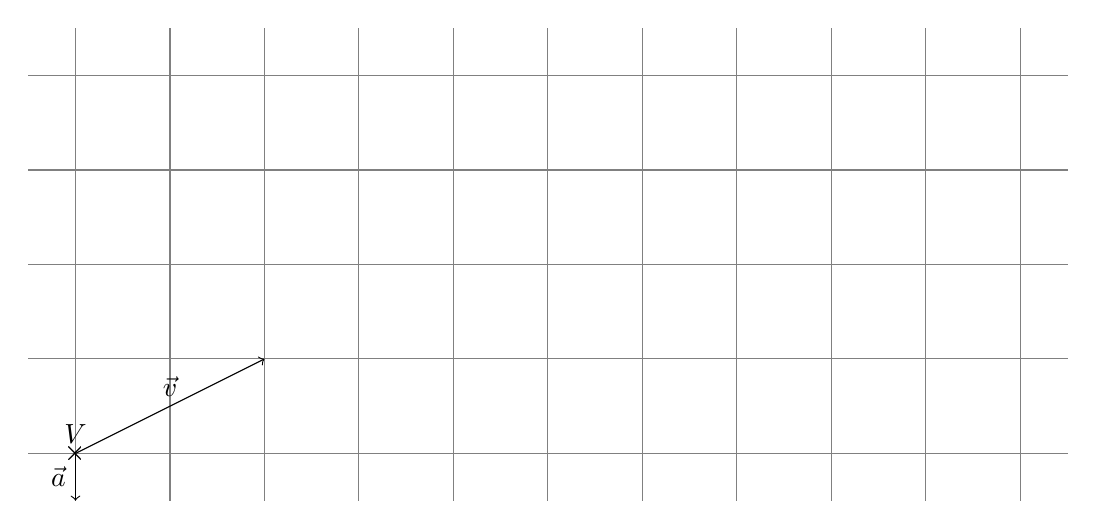
\begin{tikzpicture}[scale=1.2]
		\coordinate (AvionPosition) at (0,0);

		\draw[thin,gray] (-0.5,-0.5) grid (10.5,4.5);

		\node at (AvionPosition) {×};
		\node[above] at (AvionPosition) {$V$};
		\draw[->] (AvionPosition) -- node[above] {$\vec{v}$} ++(2,1);
		\draw[->] (AvionPosition) -- node[left] {$\vec{a}$} ++(0,-0.5);

		\ifdefined\makeCorrection
			\directlua{
			position =     { x = 0, y = 0 }
			vitesse =      { x = 2, y = 1 }
			acceleration = { x = 0, y = -0.5 }
			}

			\foreach \x in {1,...,4} {
					\directlua{
						update_position()
						update_vitesse()
						draw_position(\x, "red")
						draw_vitesse(\x, "red")
					}
				}
		\fi
	\end{tikzpicture}
\end{center}

\end{document}